\documentclass[pdftex,fontsize=12pt,a4paper,numbers=noenddot]{scrreprt}

%Beinhaltet alle verwendeten Pakete
% Dateiformat 
\usepackage[utf8]{inputenc}

% Sprache
\usepackage[ngerman]{babel}

% Silbentrennung
\usepackage[T1]{fontenc}  

% Serifenlose Schrift wie Arial
\usepackage[scaled]{uarial}
\renewcommand*{\familydefault}{\sfdefault}

% Seitenränder etc
\usepackage[left=3cm,right=3cm,top=2cm,bottom=2cm,bindingoffset=0mm]{geometry}

% Bilder und Grafiken
\usepackage{graphicx}
\usepackage{wrapfig}

% Kopf- und Fußzeilen
\usepackage{footmisc}
\usepackage[automark]{scrpage2} 

% Aufzählungen, Tabellen, ...
\usepackage{enumitem}
\usepackage{longtable}
\usepackage{supertabular}
\usepackage{tabularx}
\usepackage{longtable}
\usepackage{colortbl}
\usepackage{multirow}

% Nummerierung von Abbildungen
\usepackage{chngcntr}
\counterwithin{figure}{section}
\counterwithin{table}{section} 

% Schriftsatz
\usepackage{textcomp}
\usepackage{float}

%Abkürzungsverzeichnis
\usepackage{acronym}

% Hyperlinks in der PDF
\usepackage[colorlinks, linkcolor=black]{hyperref}
\usepackage{url}

\usepackage{pdflscape}
\usepackage{pdfpages}
% Dient zur Konfiguration von Layout und LaTeX
% Befehle zur Ausgabe von Tactical Training Team
\newcommand{\TTT}{Tactical Training Team}

% Zeilenabstand
\linespread{1.15}
\setlength{\parindent}{0pt} 

%Seitenränder
\geometry{
	left=30mm,
	right=20mm,
	top=30mm,
	bottom=30mm,
}

% Verzeichnisebenen Bilder und Tabellen
\counterwithin{figure}{section}
\counterwithin{table}{section} 

% Absand Aufzählung
\setlist[1]{itemsep=0pt}

% Farben
\usepackage{xcolor}
\definecolor{blue}{RGB}{0,0,120}
\definecolor{green}{RGB}{0,153,0}
\definecolor{backcolor}{rgb}{0.9,0.9,0.9}
\definecolor{yellow}{RGB}{255,210,0}
\definecolor{gold}{RGB}{218,165,32}
\definecolor{DarkOrchid}{RGB}{92,30,123}

% Url-Einstellungen
\hypersetup{%
	hidelinks,
	pdfauthor={\TTT}
}

% Einstellungen Kopf- und Fußzeile
\pagestyle{empty}
\clearscrheadfoot{}
\ofoot[]{\textbf{\vrule}\,\pagemark}
%\ihead[]{Tactical Training Team}
%\ohead[]{\headmark}
\chead[]{
\includegraphics[width=1.05\textwidth]{../img/header}}
\addtolength{\headheight}{10mm}
\addtolength{\footskip}{-10mm}
%\setheadsepline[\textwidth]{1pt}[\color{800000}]

% Ebenen Nummerierungen
\setcounter{secnumdepth}{4} %Nummerierungsebenen
\setcounter{tocdepth}{1}   %Ebenen Inhaltsverzeichnis

%Neuer Splatentyp für Tabellen (dient dazu, dass die erste Splate zentiert werden kann)
\newcolumntype{C}[1]{>{\centering\arraybackslash}m{#1}}
%linksbündiger Spaltentyp
\newcolumntype{P}[1]{>{\raggedright\arraybackslash}p{#1}}

%Eigenen Befehl für Newline definieren
\newcommand{\nl}{\newline}

%Autoref in Schreibmaschinenschrift
%\let\oldautoref\autoref
%\renewcommand{\autoref}[1]{\texttt{\oldautoref{#1}}}

%Nameref in Schreibmaschinenschrift und mit >> <<
\makeatletter
\shorthandon{"}
\AtBeginDocument{%
	\LetLtxMacro\oldnameref\nameref
	\DeclareRobustCommand*{\nameref}{%
		\@ifstar{\my@nameref*}{\my@nameref{}}%
	}%
	\newcommand*{\my@nameref}[2]{%
		\texttt{>>\oldnameref#1{#2}<<}%
	}%
}
\shorthandoff{"}
\makeatother

\renewcommand*{\familydefault}{\sfdefault}	
%\renewcommand*\chapterheadstartvskip {%
%	\vspace*{1\baselineskip plus .1\baselineskip minus .067\baselineskip}}

\begin{document}

\pagenumbering{gobble} %Seiten nicht mitzählen
\author{Tactical Training Team}
\begin{titlepage}
	\thispagestyle{empty}
	
\includepdf{../img/TTTitelbild.pdf}	
\end{titlepage}

\newpage
\pagenumbering{roman} %ab hier werden römischen Seiten als Seitenzahlen mitgezählt

\tableofcontents % Inhaltsverzeichnis

\newpage
\pagenumbering{arabic} %ab hier werden Seiten als Seitenzahlen mitgezählt
\pagestyle{scrheadings}
\renewcommand{\chapterpagestyle}{scrheadings}
\chapter*{Vorwort}
\addcontentsline{toc}{chapter}{Vorwort} 
\subsection*{Über dieses Dokument}
%\addcontentsline{toc}{subsection}{Über dieses Dokument} 
Entstanden aus dem ursprünglichen, kompakten Leitfaden zur Allgemeinen Grundausbildung im \ac{TTT} soll dieses Dokument sowohl Grünschnäbeln als auch Alten Hasen zum Erlernen und Festigen aller relevanten theoretischen Grundlagen des taktischen Spiels im \ac{TTT} dienen. 
Es ist Leitfaden, Referenzwerk und Messlatte in einem Dokument vereint. 
Wie jedes Schriftstück zur Ausbildung sollte es \textit{aktiv} gelesen werden: der Leserin oder der Leser sollte über die vermittelten Inhalte nachdenken, sie hinterfragen, diskutieren wo nötig und gewissenhaft einprägen.\hfil\\
Dieses Dokument lebt, es wird weiterentwickelt, überarbeitet, erweitert, gekürzt -- Anmerkungen, Vorschläge und Rückmeldungen konstruktiver Art werden nicht nur gewünscht, sondern gefordert. Ein hoher Standard im Spiel beginnt mit einem hohen Standard und Anspruch an alle Unterlagen, und jeder Spieler im \ac{TTT} ist nicht nur ständigen Verbesserung und Erweiterung seiner eigenen Fähigkeiten verpflichtet, sondern auch zur Verbesserung und Erweiterung des vermittelten Wissens.
Ein aufmerksamer, geübter Schütze mag den Ausgang eines Feuerkampfs für sich entscheiden -- der virtuelle Krieg wird jedoch durch Strategie, Taktik und das Wissen um das \textit{WIE} entschieden, das aus den Erfahrungen von Fehlschlägen und Triumphen herrührt. Der erste Schritt den du, lieber Leser, auf dem Weg zu einem erfolgreichen Spieler im \emph{[\ac{TTT}]} leisten musst, ist über diese Aussage zu meditieren und sie zu verstehen.\\

\textit{Train hard, play smart!}

\newpage
\subsection*{Die Grundsätze des TTT}
\label{sec:Grundsaetze}
%\addcontentsline{toc}{subsection}{Die Grundsätze des TTT} 
	\begin{itemize}
		\item Das [TTT] stellt das Training in den Mittelpunkt
		\item Das [TTT] spielt auf höchstem taktischen Niveau
		\item Das [TTT] orientiert sich in seiner Spielweise und Organisation an Kommando-Teams
		\item Das [TTT] pflegt und lebt das Battle Buddy System
		\item Das [TTT] lässt im Spiel keinen Kamerad zurück, jedem Notruf wird Folge geleistet
		\item Das [TTT] ist eine offene Community -- jeder kann am Training oder den Events grundsätzlich teilnehmen
		\item Die [TTT] Community wird geführt wie ein aktives, ergebnisorientiertes Unternehmen -- die Stammspieler sind das wichtigste Kapital	
	\end{itemize}

\vspace*{\fill}
	\today
	\begin{figure}[htbp]
		
\includegraphics{../img/by-nc-sa}
	\end{figure}

Some pictures and graphics of this document was created using ARMA 3.\\
ARMA 3 is a registered trademark of Bohemia Interactive a.s.\\
See www.bistudio.com for more information.

\part{}
%Truppengattungen
\pagebreak
\section{Verhalten bei Feindkontakt}
Wird ein Feind ausgemacht, so meldet ein Truppmitglied diesen an den TF.\\

Dies könnte im Truppfunk so gemeldet werden:\\
>>1 hier 6, Kontakt, stationäres MG auf 290°, Entfernung ca. 800\,m, Kalt<<

Eine andere Situation ergibt sich wenn der Feind das Feuer auf die eigene Stellung eröffnet. Hier hängt es von der Ausgabe des Feuerstatus ab. Ist Feuerstatus rot ausgegeben wird das Feuer nur erwidert wenn es ums blanke überleben geht.\\

Hier kommen die Kommandos >>Stellung wechseln<<, >>Feuer Frei<<, >>Ausweichen<< oder >>Verzögern und Ausweichen<< in Frage.\footnote{Ausführlich in >>\nameref{sec:kommando}<< beschrieben}\\

In allen fällen gibt der TF das Kommando aus, wie sich verhalten werden soll.

% Grundlagen
\pagebreak
\section{Verhalten bei Feindkontakt}
Wird ein Feind ausgemacht, so meldet ein Truppmitglied diesen an den TF.\\

Dies könnte im Truppfunk so gemeldet werden:\\
>>1 hier 6, Kontakt, stationäres MG auf 290°, Entfernung ca. 800\,m, Kalt<<

Eine andere Situation ergibt sich wenn der Feind das Feuer auf die eigene Stellung eröffnet. Hier hängt es von der Ausgabe des Feuerstatus ab. Ist Feuerstatus rot ausgegeben wird das Feuer nur erwidert wenn es ums blanke überleben geht.\\

Hier kommen die Kommandos >>Stellung wechseln<<, >>Feuer Frei<<, >>Ausweichen<< oder >>Verzögern und Ausweichen<< in Frage.\footnote{Ausführlich in >>\nameref{sec:kommando}<< beschrieben}\\

In allen fällen gibt der TF das Kommando aus, wie sich verhalten werden soll.

%Fortgeschrittenes
\pagebreak
\section{Verhalten bei Feindkontakt}
Wird ein Feind ausgemacht, so meldet ein Truppmitglied diesen an den TF.\\

Dies könnte im Truppfunk so gemeldet werden:\\
>>1 hier 6, Kontakt, stationäres MG auf 290°, Entfernung ca. 800\,m, Kalt<<

Eine andere Situation ergibt sich wenn der Feind das Feuer auf die eigene Stellung eröffnet. Hier hängt es von der Ausgabe des Feuerstatus ab. Ist Feuerstatus rot ausgegeben wird das Feuer nur erwidert wenn es ums blanke überleben geht.\\

Hier kommen die Kommandos >>Stellung wechseln<<, >>Feuer Frei<<, >>Ausweichen<< oder >>Verzögern und Ausweichen<< in Frage.\footnote{Ausführlich in >>\nameref{sec:kommando}<< beschrieben}\\

In allen fällen gibt der TF das Kommando aus, wie sich verhalten werden soll.

%Mods
\part{SGA \& Tutorials}
%\chapter{Gepanzerte Fahrzeuge}
\section{Der Schützenpanzer}
	Ein Schützenpanzer ist ein leicht gepanzertes Fahrzeug, welches das Bindeglied zwischen leichten Transportfahrzeugen und schweren Panzern darstellt. Primär dient ein SPz zur Unterstützung von verbündeten Infanteriekräften sowohl im urbanen- als auch im offenen Gelände. Innerhalb des Schützenpanzers bilden speziell ausgebildete Infanteriekräfte die Nahsicherung des Fahrzeuges, welche in einem späteren Kapitel näher erläutert werden.\\
	
	In Arma 3 stehen viele verschiedene Modelle eines SPz zur Verfügung, diese unterscheiden sich in Dingen wie:
	\begin{itemize}
		\item Fassungsvermögen von Infanterie
		\item Bewaffnung
		\item Visierung
		\item Ketten- sowie Radpanzer
	\end{itemize}
	
	In der folgenden Übersicht werden verschiedene Modelle präsentiert und ihre jeweiligen Spezifikationen aufgelistet.

\subsection{Modfahrzeuge}
	\begin{longtable}{lc} 
		\toprule
		Bradley (Blufor) & \multirow{2}{*}{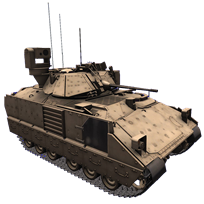
\includegraphics[width=0.4\textwidth]{./img/tutorials/spz/bradley}}\\
		\begin{minipage}[t]{0.4\textwidth}
			\begin{itemize}
				\item Platz für 9 Mann (3 Besatzung, 6 Infanteristen)
				\item Bewaffnung:
				\begin{itemize}
					\item 25 mm Bordkanone
					\item 7.62 mm koaxial MG
					\item TOW AT Raketen
				\end{itemize}
				\item Nebelmittelwurfanlage
				\item Kettenfahrzeug
			\end{itemize}
		\end{minipage}\\
		\midrule
		Puma (Blufor) & \multirow{2}{*}{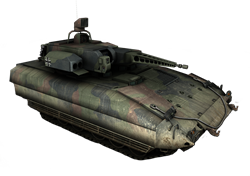
\includegraphics[width=0.4\textwidth]{./img/tutorials/spz/puma}}\\
		\begin{minipage}[t]{0.4\textwidth}
			\begin{itemize}
				\item Platz für 9 Mann (3 Besatzung, 6 Infanteristen)
				\item Bewaffnung:
				\begin{itemize}
					\item 30 mm Bordkanone
					\item 7.62 mm koaxial MG
					\item Spike AT Raketen
				\end{itemize}
				\item Nebelmittelwurfanlage
				\item Kettenfahrzeug
			\end{itemize}
		\end{minipage}\\	
		\bottomrule 
	\end{longtable}

\section{Bewaffnung und Panzerung von Schützenpanzer}
Schützenpanzer sind durch ihre modulare Bauweise in Sachen Bewaffnung und Panzerung äußerst flexibel aufrüstbar.

\subsection{Bewaffnung}
	Im Militär werden gegnerische Feindkräfte in Bezug auf Panzerung in drei Klassen unterteilt:
	\begin{longtable}{ll} 
		\toprule
		Typ & Definition\\
		\midrule
		Weich & Nicht gepanzerte Kräfte wie Infanterie, Transportfahrzeuge, etc.\\
		Halb-Hart & Leicht gepanzerte Ziele wie Schützenpanzer.\\
		Hart & Schwer gepanzerte Ziele wie Kampfpanzer.\\
		\bottomrule 
	\end{longtable}

	Standardmäßig ist ein Schützenpanzer mit einer Bordkanone, einem Maschinengewehr sowie einer Feuerleitanlage ausgestattet, welche eine effektive Bekämpfung feindlicher Panzerkräfte ermöglicht.
	\begin{longtable}{ll} 
		\toprule
		Waffensystem & Zieltyp\\
		\midrule
		\multirow{2}{*}{Bordkanone} & Weich\\
		& Halb-Hart\\
		Maschinengewehr (Koaxial) & Weich\\
		\multirow{2}{*}{Granatwerfer} & Weich\\
		& Halb-Hart\\
		\bottomrule 
	\end{longtable}

\subsection{Panzerung}
	Schützenpanzer bieten in der Realität eine meist gut ausgebaute Panzerung, welche so in ArmA jedoch nicht implementiert wurde. Folgende Punkte sollten im Kampfgeschehen beachtet werden.\\

	Ein SPz ist gegen Handfeuerwaffen nahezu vollständig geschützt, bietet gegen Beschuss von mobiler Panzerabwehr jedoch nur bedingt Schutz. Dies ist von der Position des Einschlags des Projektils sowie Entfernung abhängig.\\
	Beschuss durch feindliche, harte Kräfte enden meist in einem Totalverlust des Fahrzeuges, sodass eine Konfrontation mit diesen Kräften um jeden Preis vermieden werden sollte.\\

	Daher ist zu empfehlen, den Schützenpanzer nur als Unterstützungselement einzusetzen (siehe Bild) und durch verbündete, abgesessene Infanterie, im Nahbereich zu sichern.\\
	\begin{figure}[htbp]
		\centering
		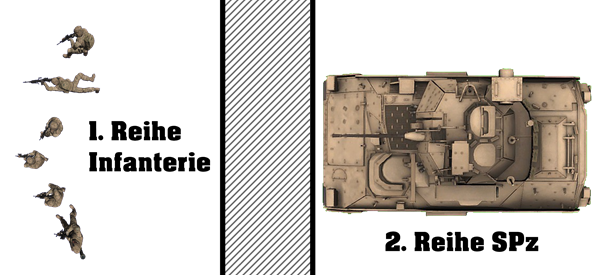
\includegraphics[width=0.95\linewidth]{./img/tutorials/spz/reihe}
		\caption{Sicherungspostionen Infanterie und SPz}
	\end{figure}

\section{Der Kampfpanzer}
	Der Kampfpanzer (kurz KPz) ist ein schwer gepanzertes Fahrzeug, welches primär zur Bekämpfung von harten Zielen eingesetzt wird, jedoch ebenso bestens für eine Bekämpfung weichen / halb-harten Zielen geeignet ist.\\

	In Arma 3 stehen viele verschiedene Modelle eines KPz zur Verfügung, welche sich in Bewaffnung / Visierung / Panzerung unterscheiden.\\
	In der folgenden Übersicht werden verschiedene Modelle mit ihren jeweiligen Spezifikationen aufgelistet.\\

\subsection{Modfahrzeuge}
\subsection{Vanilla Arma 3 Fahrzeuge}

\section{Bewaffnung und Panzerung von Kampfpanzer}
\subsection{Bewaffnung}
	Alle Kampfpanzer in Arma 3 sind mit einer Glattrohrkanone und einem leichten bis schweren Maschinengewehr ausgerüstet. Die Glattrohrkanone kann wahlweise mit einem HE- (High Explosive) oder einem AP- (Armor Piercing) Geschoss geladen werden.
	\begin{longtable}{ll} 
		\toprule
		Waffensystem & Zieltyp\\
		\midrule
		\multirow{3}{*}{Glattrohrkanone} & Weich (HE)\\
		& Halb-Hart (AP)\\
		& Hart (AP)\\
		Maschinengewehr (Koaxial) & Weich\\
		\bottomrule 
	\end{longtable}

\subsection{Panzerung}
	Die Hauptpanzerung des Fahrzeuges bietet vollständigen Schutz gegenüber Beschuss von Handfeuerwaffen. Potentielle Gegner des Kampfpanzers stellen schwere Feindkräfte wie Jets, Helikopter, SPz, KPz und spezialisierte Infanterietruppen dar. Diese können, bedingt durch ihre spezialisierten Anti-Panzer-Bewaffnungen, immensen Schaden am Fahrzeug ausrichten, bis hin zum Totalverlust des Fahrzeuges. 

\section{Die Crew}
\label{sec:panzercrew}
	Die Crew ist das wichtigste Element eines Panzerfahrzeuges und bildet somit das Herzstück dieser Einheit. Nur eine eingespielte Besatzung kann das Fahrzeug effektiv einsetzen und so das Kampfgeschehen im entscheidenden Moment beherrschen.\\
	Hierbei ist die Kommunikation der wichtigste Faktor und sollte nicht unterschätzt werden, im Ernstfall entscheiden wenige Sekunden über Leben und Tod der Besatzung.\\

	Eine erfolgreich eingespielte Crew zeichnet sich dadurch aus, dass in der Kampfphase nurnoch wenige Worte gesprochen werden müssen, da eine Vielzahl der nötigen Befehle bereits in einen Automatismus übergegangen sind. Gegenseitiges, uneingeschränktes Vertrauen in die jeweils anderen ist hier unumgänglich.\\

	Jedem Posten innerhalb des Panzerfahrzeuges sind spezielle Aufgaben zugewiesen, welche in der folgenden Tabelle näher erläutert werden.

\subsection{Die Aufgaben der Crew}
	\begin{longtable}{lp{0.5\textwidth}} 
		\toprule
		\multirow{2}{*}{Kommandant} & Zentrales Führungselement des Fahrzeuges\\
		& \begin{minipage}[t]{0.4\textwidth}
			Aufgaben:
			\begin{itemize}
				\item Führen des Panzerfahrzeuges
				\item Oberbefehl über die Infanterie
				\item Gesamtüberblick behalten
				\item Kommunikation mit anderen Einheiten
			\end{itemize}
		\end{minipage}\\
		\midrule
		\multirow{2}{*}{Richtschütze} & Bedienung der Waffenanlage\\
		& \begin{minipage}[t]{0.4\textwidth}
			Aufgaben:
			\begin{itemize}
				\item Bedienung der Waffenanlage
				\item Überwachung der Umgebung
				\item Feindkontakt melden
				\item Einweisen des Fahrers
			\end{itemize}
		\end{minipage}\\	
		\midrule
		\multirow{2}{*}{Kraftfahrer} & Steuerung des Fahrzeuges\\
		& \begin{minipage}[t]{0.4\textwidth}
			Aufgaben:
			\begin{itemize}
				\item Sicheres Manövrieren des Fahrzeuges
				\item Ausführen der Befehle
				\item Feindkontakt melden
			\end{itemize}
		\end{minipage}\\		
		\bottomrule 
	\end{longtable}
	
\section{Steuerung und Befehle}
	In diesem Kapitel wird anhand von Beispielen die Steuerung- und Befehlsstruktur zur Führung eines Panzerfahrzeuges erklärt.
	
\subsection{Fahrer: Steuerung, Befehle und Hinweise}
\subsubsection{Steuerung}
	\begin{longtable}{ll} 
		\toprule
		Steuerung & Tasten\\
		\midrule
		Fahrzeug steuern & \keys{W}, \keys{A}, \keys{S}, \keys{D}\\
		Schnell fahren & \keys{Shift + W}\\
		Langsam fahren & \keys{Strg + W}\\
		Luke auf\,/\,Luke zu & \keys{Strg + Q}\,/\,\keys{Strg + E}\\
		Handbremse (nur bei Radfahrzeugen) & \keys{X}\\
		Geschwindigkeitsbegrenzer an\,/\,aus & \keys{Entf}\\
				\bottomrule 
	\end{longtable}	
	
\subsubsection{Befehle}
	Wie bereits in Kapitel \ref{sec:panzercrew} \nameref{sec:panzercrew} angemerkt, ist die Kommunikation im Fahrzeug äußerst wichtig. Deshalb beschränkt sich die Kommunikation zwischen Kommandant und Fahrer auf kurze, prägnante Befehle, wie es den folgenden Beispielen zu entnehmen ist.

	\begin{longtable}{p{0.45\textwidth}p{0.5\textwidth}} 
		\toprule
		Kommando & Ausführung\\
		\midrule
		„Crew  Befehl  Hinweis“ & Die Kommandos sind modular aufgebaut und können entsprechend, je nach Situation, abgeändert werden.\\
		\midrule
		Den Panzer auf der Stelle (stehend) ausrichten (drehen).\vspace{6pt}\nl
		„Fahrer ausrichten 1-1-0 Grad“
		& Fahrer dreht die Panzerwanne in Kompassrichtung 1-1-0 Grad\\
		\midrule
		Den Panzer mit Richtgeschwindigkeit in Bewegung setzen.\vspace{6pt}\nl
		Fahrer vorwärts 2-2-0 Grad, 30 Km/h“
		& Kommando “Vorwärts” wird genutzt, um individuelle Geschwindigkeiten vorzugeben.\\
		\midrule
		Den Panzer in Bewegung setzen.\vspace{6pt}\nl
		„Fahrer Marsch 2-2-0 Grad“
		& Fahrer fährt mit verminderter Geschwindigkeit nach vorne (Strg + W), in Kompassrichtung 2-2-0 Grad.\\
		\midrule
		Den Panzer schnell in Bewegung setzen.\vspace{6pt}\nl
		„Fahrer  Marsch Marsch 2-2-0 Grad“
		& Fahrer fährt in normaler Geschwindigkeit (W) in Richtung 2-2-0 Grad\\
		\midrule
		Den Panzer schnellst möglich fahren.\vspace{6pt}\nl
		„Fahrer Sprung 2-2-0 Grad, Straße folgen.
		& Fahrer fährt mit Höchstgeschwindigkeit (Shift+W) in Richtung 2-2-0 Grad, und folgt der Straße.\\
		\midrule
		Den Panzer anhalten\vspace{6pt}\nl
		„Fahrer anhalten“
		& Der Fahrer bremst seinen Panzer sanft bis zum Stillstand.\\
		\midrule
		Den Panzer sofort zum stehen bringen.\vspace{6pt}\nl
		„Fahrer STOP“
		& Der Fahrer führt eine Vollbremsung aus. (Im Konvoi wegen hoher Unfallgefahr vermeiden)\\		 
		\bottomrule 
	\end{longtable}	
%\pagebreak
\section{Verhalten bei Feindkontakt}
Wird ein Feind ausgemacht, so meldet ein Truppmitglied diesen an den TF.\\

Dies könnte im Truppfunk so gemeldet werden:\\
>>1 hier 6, Kontakt, stationäres MG auf 290°, Entfernung ca. 800\,m, Kalt<<

Eine andere Situation ergibt sich wenn der Feind das Feuer auf die eigene Stellung eröffnet. Hier hängt es von der Ausgabe des Feuerstatus ab. Ist Feuerstatus rot ausgegeben wird das Feuer nur erwidert wenn es ums blanke überleben geht.\\

Hier kommen die Kommandos >>Stellung wechseln<<, >>Feuer Frei<<, >>Ausweichen<< oder >>Verzögern und Ausweichen<< in Frage.\footnote{Ausführlich in >>\nameref{sec:kommando}<< beschrieben}\\

In allen fällen gibt der TF das Kommando aus, wie sich verhalten werden soll.
%\pagebreak

%Sonstiges
\chapter{Sonstiges}
%%\begin{landscape} %Querformat
\section{nützliche Tastatur (Um)Belegung}
Tipp: Kompass auf >>Leertaste<< legen so ist dieser leichter verfügbar als über die Taste >>K<<
%\end{landscape}
%das Abkürzungsverzeichnis erstellen
\pagebreak
\chapter*{Abkürzungsverzeichnis}
\addcontentsline{toc}{chapter}{Abk\"urzungsverzeichnis} 
\begin{acronym}[SEPSEPSEP]
\setlength{\itemsep}{1em}
	\acro{AAR}{After Action Report}
	\acro{OPL}{Operationsleitung}
	\acro{SQL}{Squadlead}
	\acro{FAC}{Forward Air Controler}
	\acro{AT}{Anti Tank}
	\acro{UAV}{Unmanned Aerial Vehicle}
	\acro{TTT}{Tactical Training Team}
	\acro{AA}{Anti Air}
	\acro{KPZ}{Kampfpanzer}	
	\acro{SPZ}{Schützenpanzer}
	\acro{CAS}{Close Air Support}
	\acro{CQB}{Operationsleitung}
	\acro{AGA}{Allgemeine Grundausbildung}
	\acro{SGA}{Spezielle Grundausbildung}
	\acro{KSK}{Kommando Spezialkräfte}
	\acro{MedEvac}{MEDical EVACuation}
	\acro{CSE}{Combat Space Enhancement}
	\acro{IR}{Infrarot}
	\acro{EOD}{Explosive Ordnance Disposal}
	\acro{LZ}{Landezone}
	\acro{KT}{Kampftrupp}
	\acro{SR}{Short Range}
	\acro{LR}{Long Range}
	\acro{MG}{Maschinengewehr}
\end{acronym}
\pagebreak

%Ganz zum Schluss
\pagebreak
\chapter*{Autoren}
\addcontentsline{toc}{chapter}{Autoren} 
	Ein herzliches Dank an euch für eure fleißige Mitarbeit, sowie an alle die am \ac{TTT} mitwirken. 
	\par\bigskip
	\begin{tabular}{p{0.23\textwidth}p{0.23\textwidth}p{0.23\textwidth}p{0.23\textwidth}}
		Ghost & 
		grauer Wolf &
		Grunt &
		GSG9\_abzocker\\
		Highhead &
		LingLing & 
		Lorddrinkalot &
		Lufros\\
		Mynx &
		Nachti &
		Reimchen &
		Relain\\
		Schotte &
		SCiite &
		Speutzi &
		Stura \\
		TheConen\\
	\end{tabular}	

\cleardoublepage
\appendix
\end{document}